\begin{figure}[ht]
    \centering
    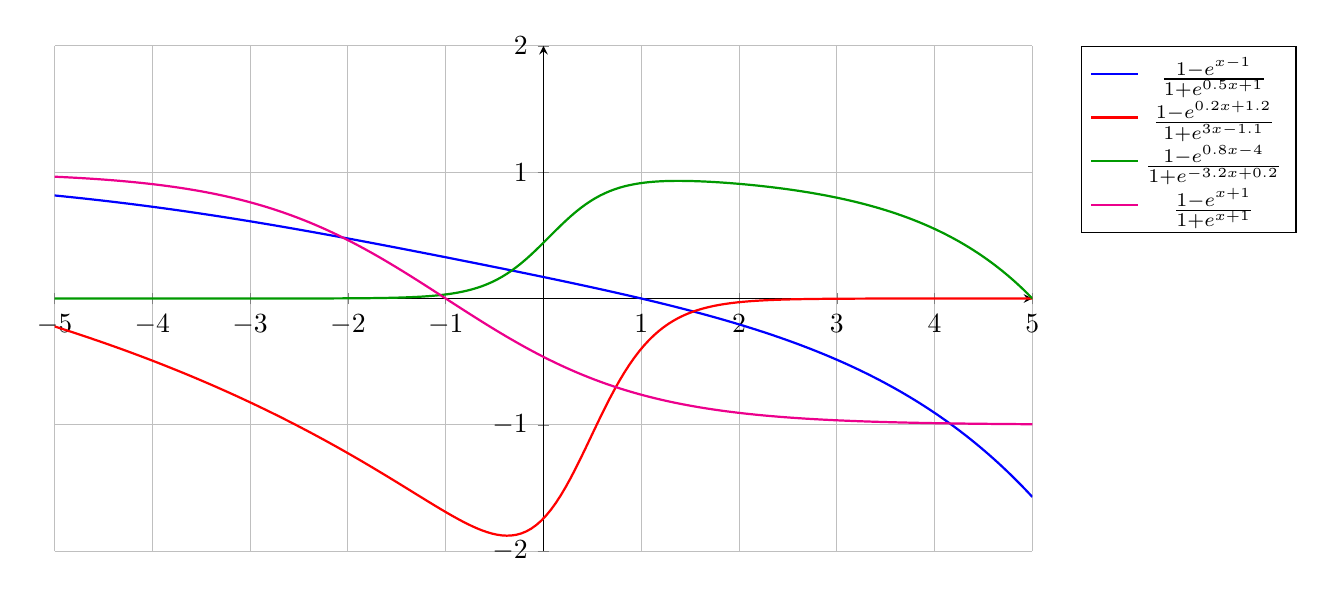
\begin{tikzpicture}
        \begin{axis}[
            width=14cm,
            height=8cm,
            xmin=-5, xmax=5,
            ymin=-2, ymax=2,
            axis lines=middle,
            grid=both,
            legend style={at={(1.05,1)},anchor=north west}
        ]
        % 1. [1, -1, 0.5, 1]
        \addplot[
            domain=-5:5, 
            samples=200, 
            thick, 
            blue
        ]
        {(1 - exp(1*x - 1)) / (1 + exp(0.5*x + 1))};
        \addlegendentry{$\frac{1 - e^{x - 1}}{1 + e^{0.5x + 1}}$}
        
        % 2. [0.2, 1.2, 3, -1.1]
        \addplot[
            domain=-5:5, 
            samples=200, 
            thick, 
            red
        ]
        {(1 - exp(0.2*x + 1.2)) / (1 + exp(3*x - 1.1))};
        \addlegendentry{$\frac{1 - e^{0.2x + 1.2}}{1 + e^{3x - 1.1}}$}
        
        % 3. [0.8, -4, -3.2, 0.2]
        \addplot[
            domain=-5:5, 
            samples=200, 
            thick, 
            green!60!black
        ]
        {(1 - exp(0.8*x - 4)) / (1 + exp(-3.2*x + 0.2))};
        \addlegendentry{$\frac{1 - e^{0.8x - 4}}{1 + e^{-3.2x + 0.2}}$}
        
        % 4. [1, 1, 1, 1]
        \addplot[
            domain=-5:5, 
            samples=200, 
            thick, 
            magenta
        ]
        {(1 - exp(1*x + 1)) / (1 + exp(1*x + 1))};
        \addlegendentry{$\frac{1 - e^{x + 1}}{1 + e^{x + 1}}$}
        
        \end{axis}
    \end{tikzpicture}
    \caption{Функции активации на основе REAct \eqref{eq:react}}
    \label{fig:react_func_graph}    
\end{figure}